\section{Durchführung}
\label{sec:Durchführung}

Der Versuch besteht aus zwei Teilen, welche aus einer Niedrig- und einer Hochdruck-Messreihe bestehen.
\subsection{Druckbereich von 30 bis 1000\,mbar}
In diesem Teil des Versuchs wird die Dampfdruckkurve von Wasser zwischen 30 bis 1000 mbar bestimmt.
Eine Wasserstrahlpumpe ist über die Woulffsche Flasche (zu sehen in Abbildung 3) mit dem Rest der Apparatur verbunden.
Diese Flasche lässt sich durch einen Absperrhahn und ein Drosselventil abriegeln.\\ 
\begin{figure}[H]
    \begin{subfigure}{0.45\textwidth}
    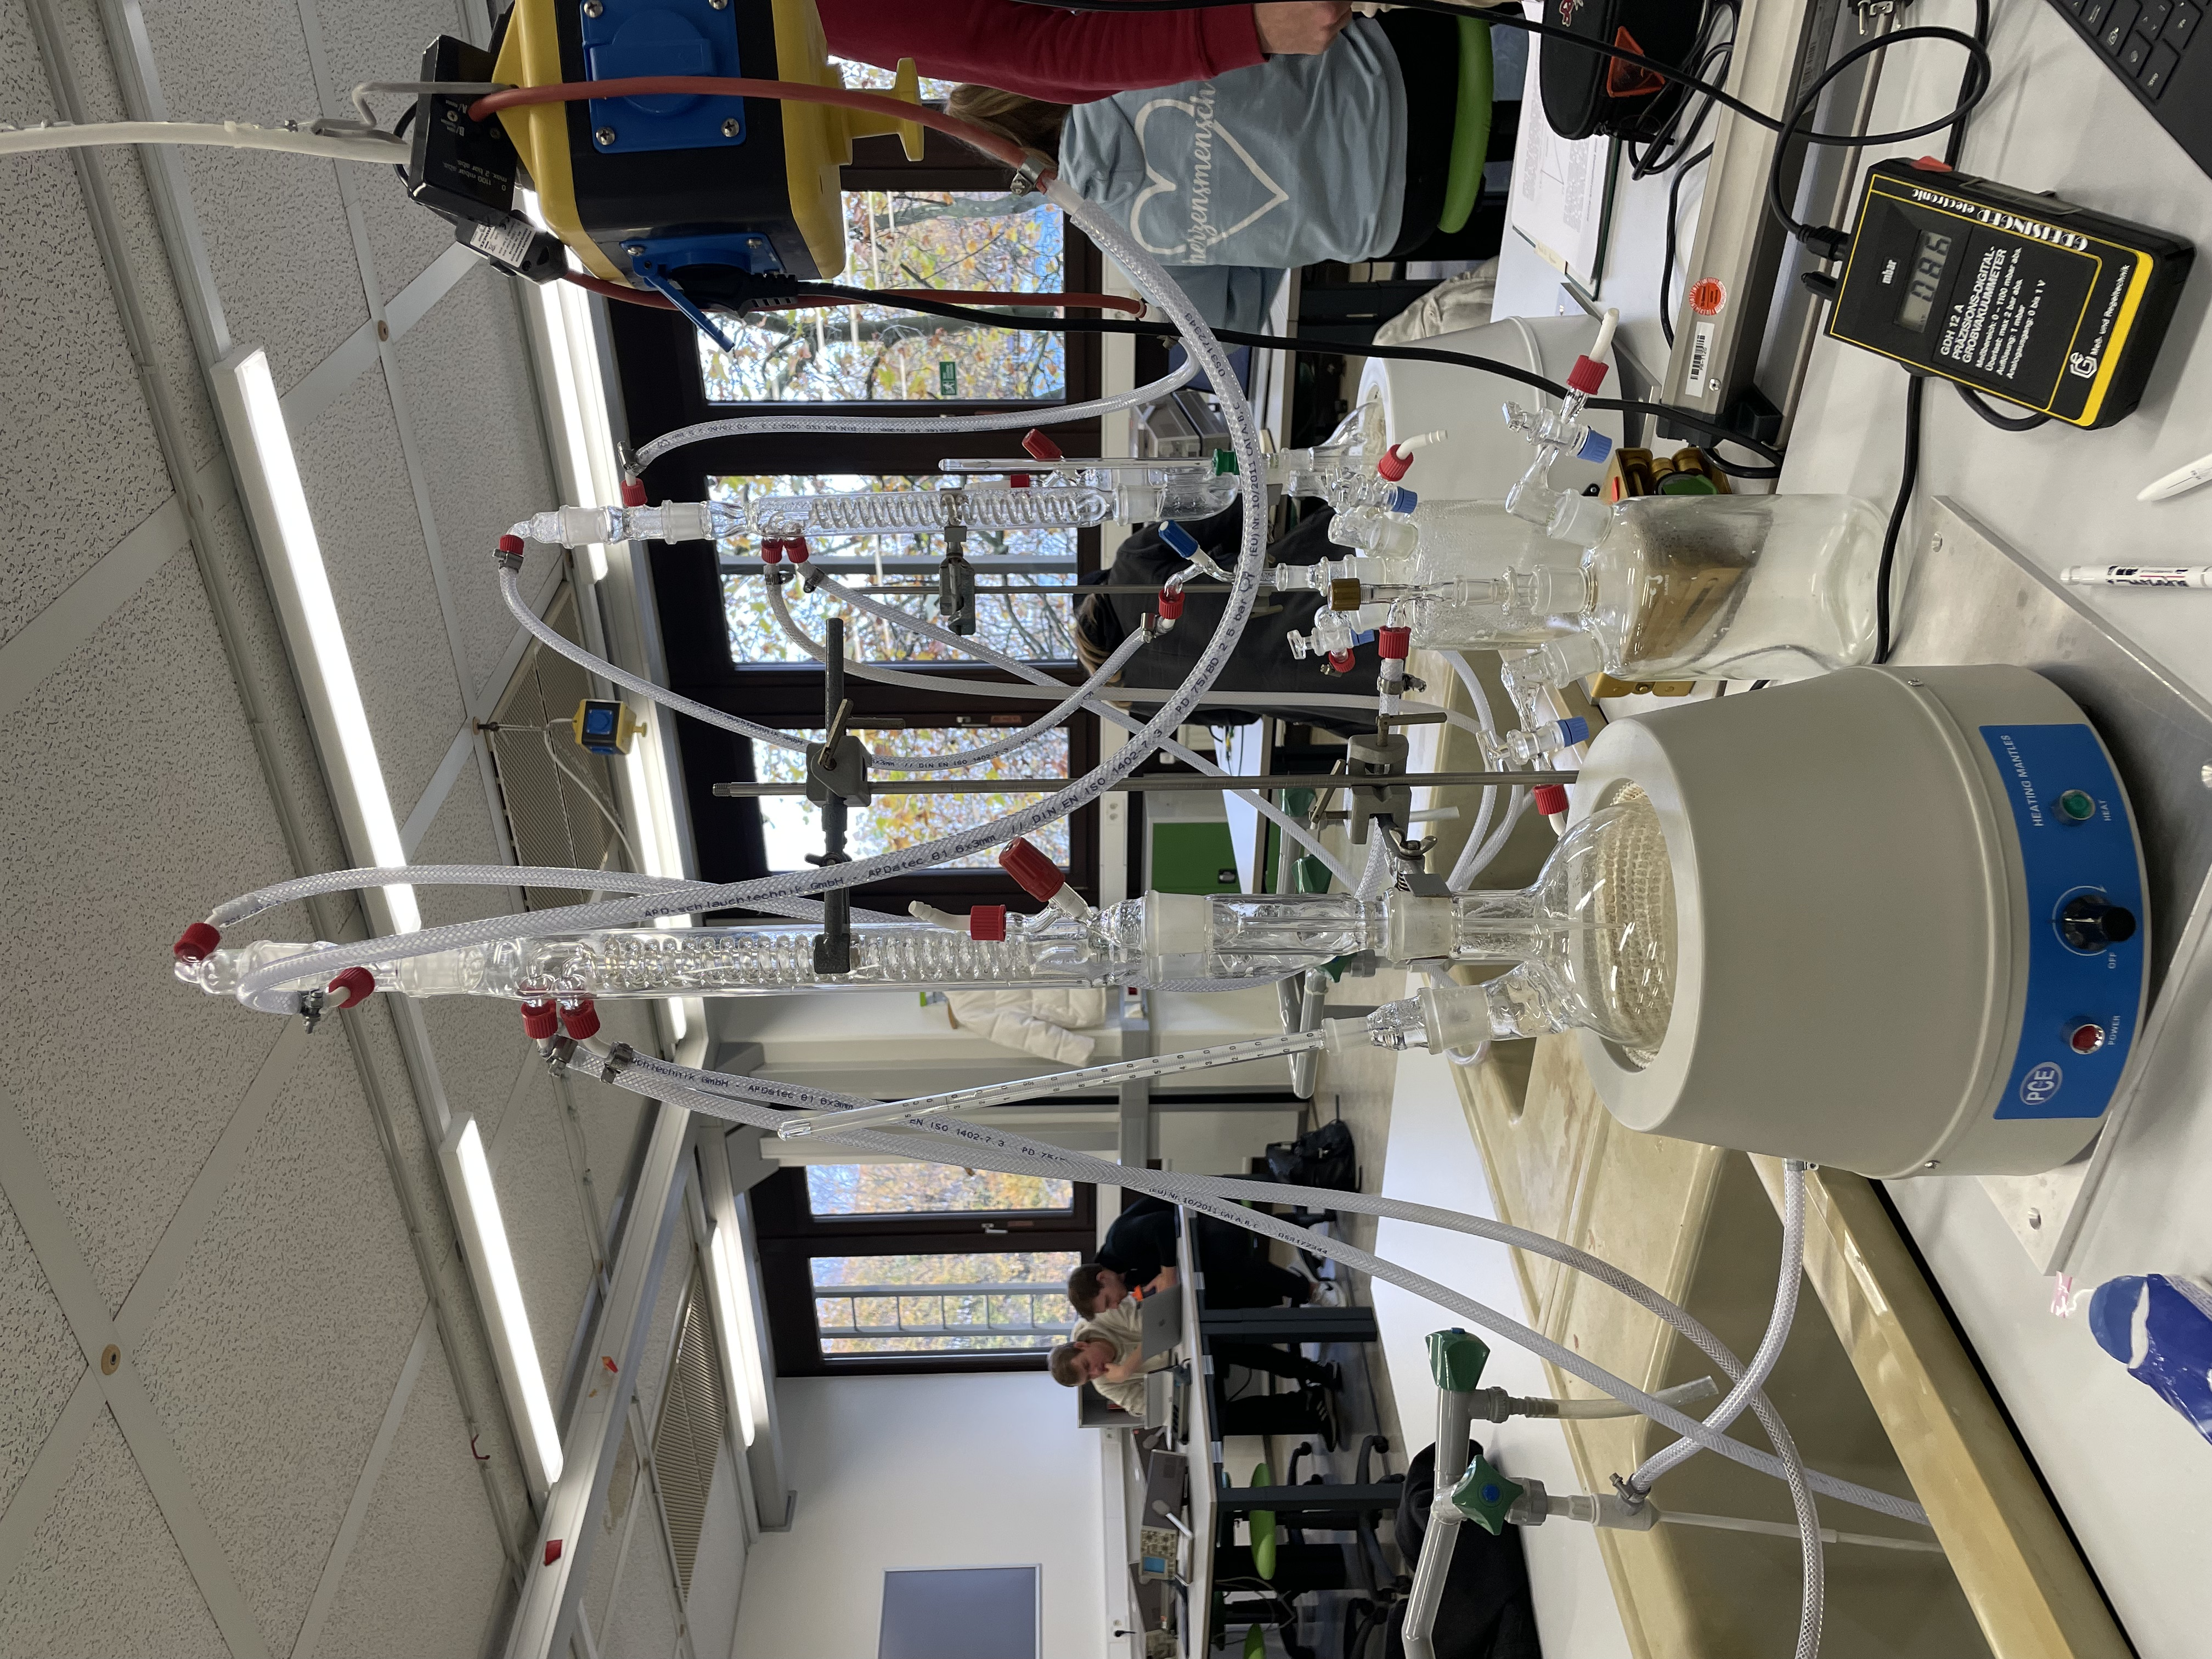
\includegraphics[angle=270,scale=0.05]{content/Verwendete_Messapparatur.jpeg}
    \label{Abb:Messapparatur}
    \end{subfigure}
    \hfill
    \begin{subfigure}{0.45\textwidth}
    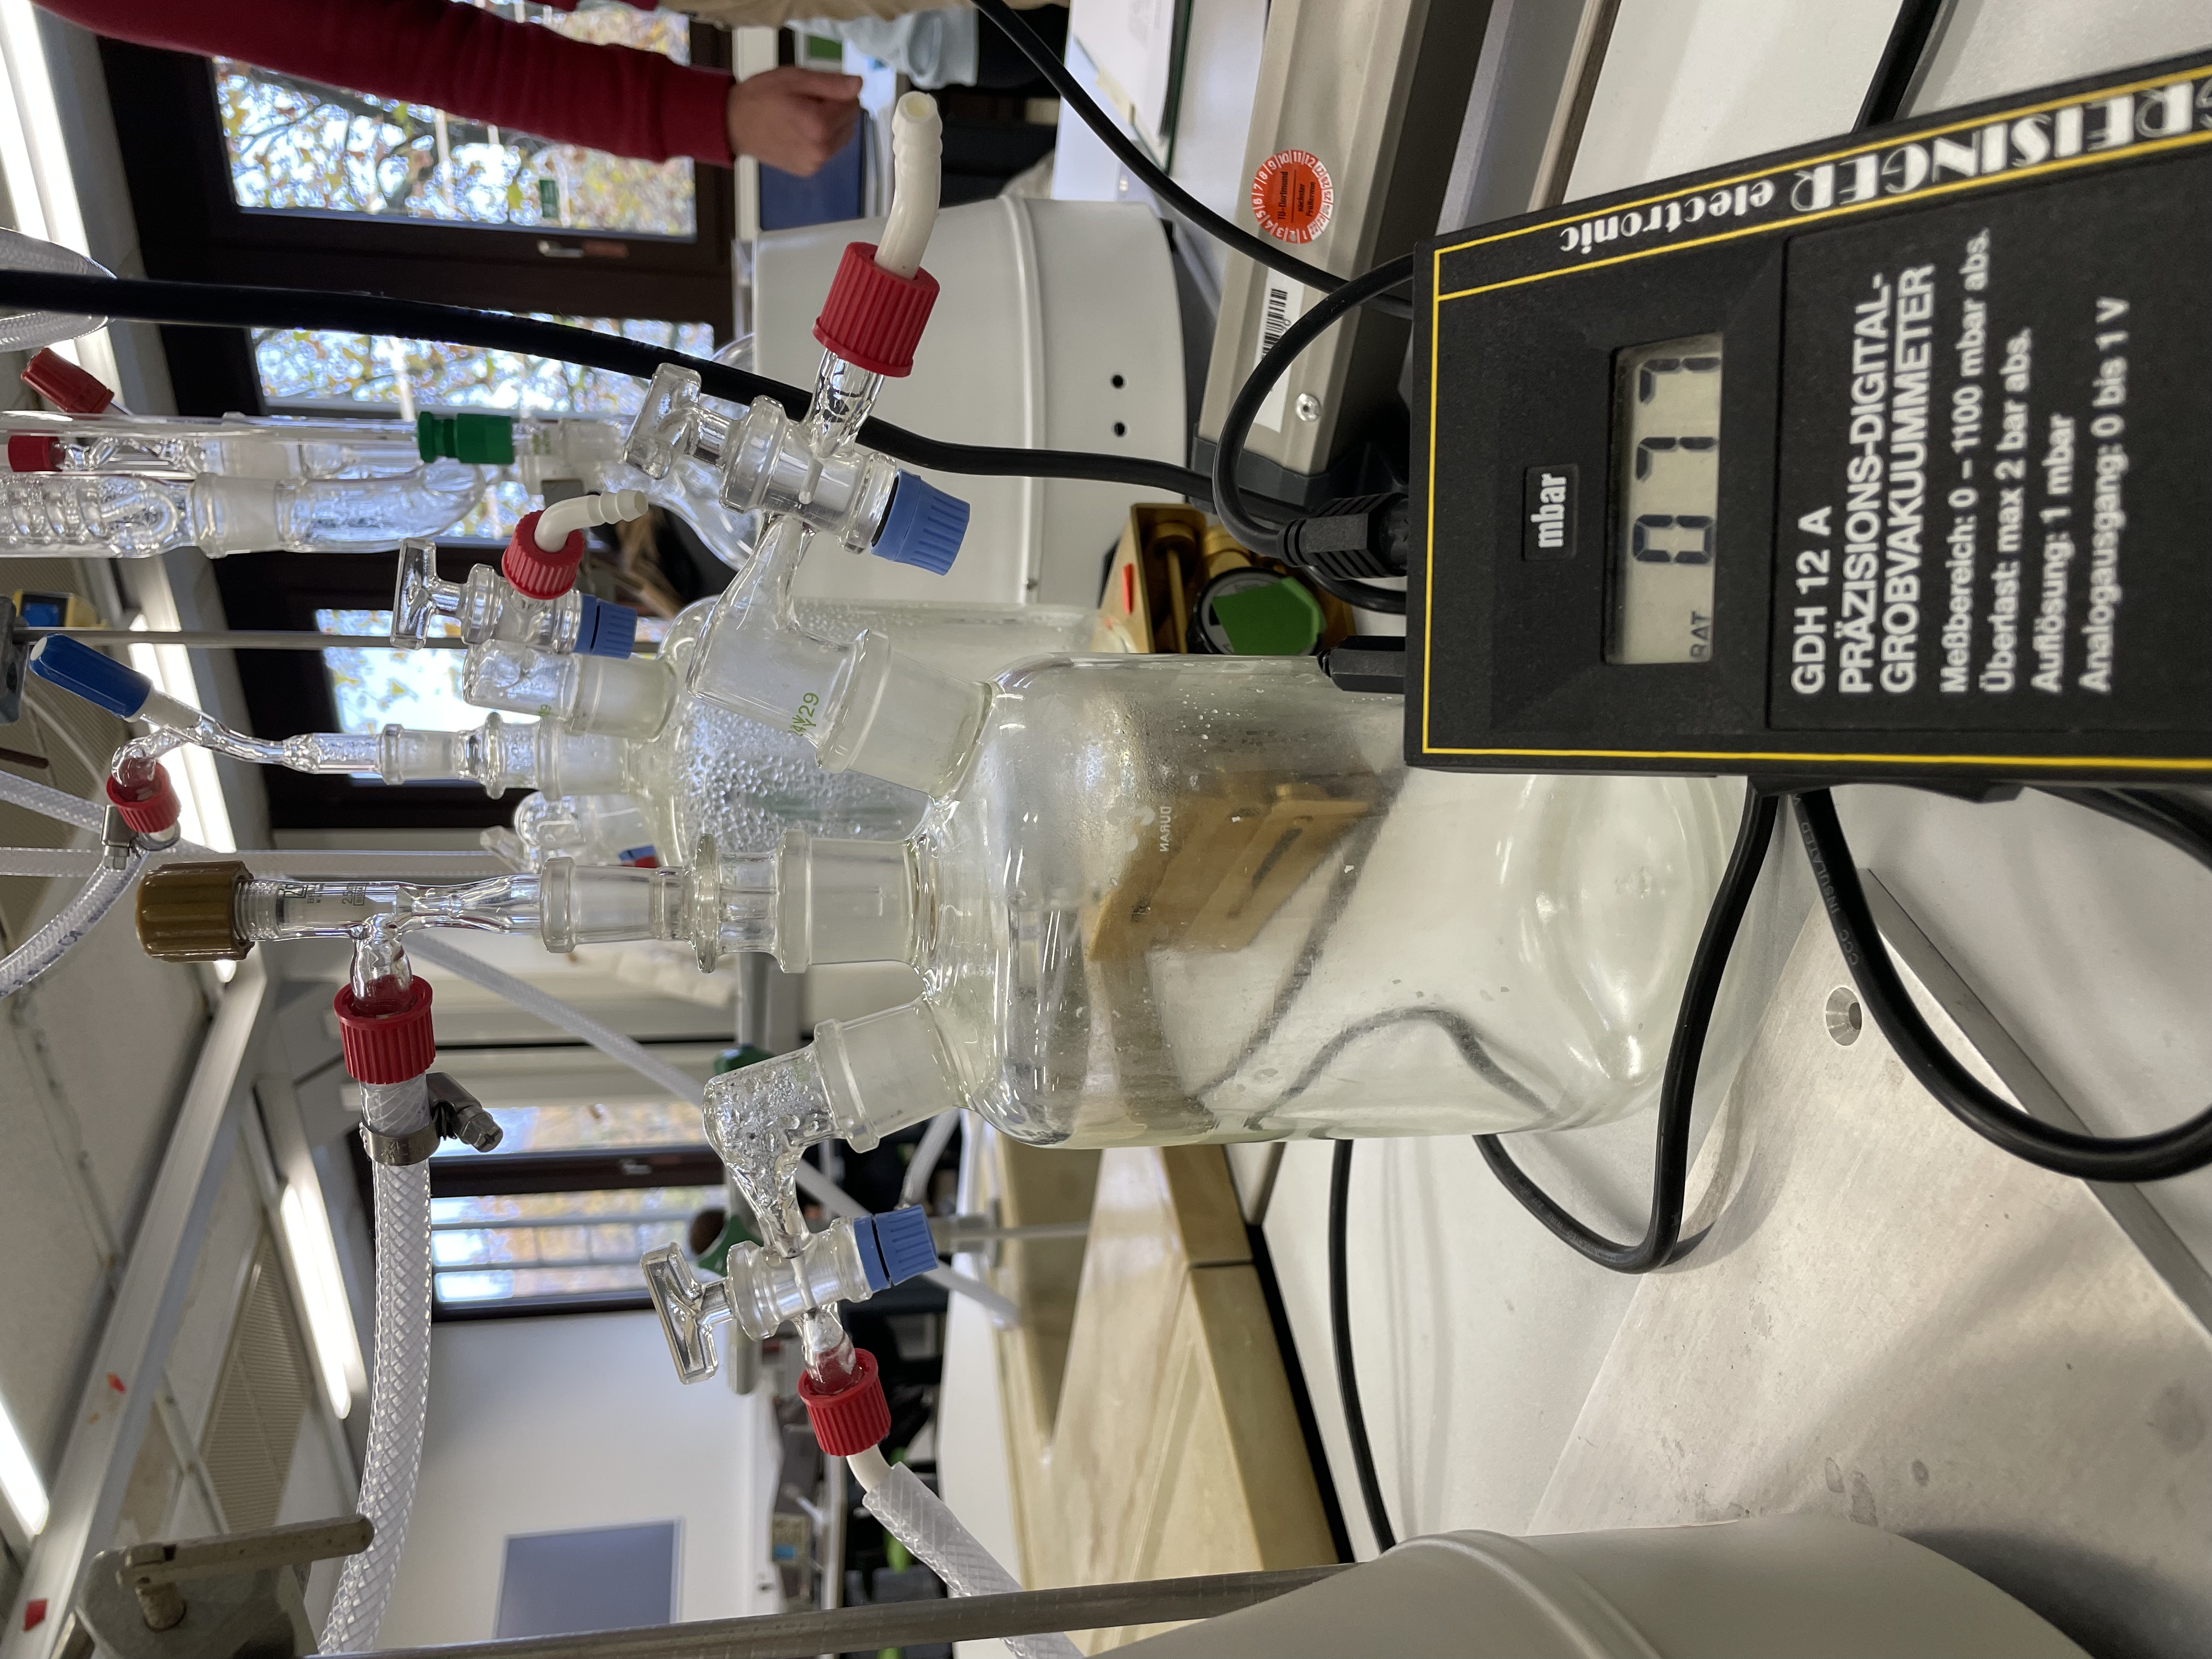
\includegraphics[angle=270,scale=0.05]{content/Woulffsche_Flasche.jpeg}
    \label{Abb:Woulffsche_Flasche}
    \end{subfigure}
    \caption{Die Messapparatur für den Tiefdruck-Messbereich.}
\end{figure}\noindent
Ein Manometer ist ebenfalls mit dem Mehrhalskolben verbunden, um kontinuierlich den Dampfdruck im Inneren messen zu können.
Er ist in Abbildung 3 auf der linken Abbildung zu sehen.
Der Mehrhalskolben wird von einer Heizhaube, auf der er steht, erhitzt.
In diesem Kolben befindet sich das zu erhitzende Wasser.
Außerdem befindet sich im Kolben ein Thermometer, so kann die Temperatur zu jeder Zeit abgelesen werden.
Ein Rückflusskühler macht die Messapparatur komplett.
Er lässt die aufsteigenden Dämpfe kondensieren, damit sich nicht in das Manometer gelangen.
\noindent
Zunächst wird die ganze Apparatur mittels der Wasserstrahlpumpe evakuiert, bis der Druck auf 30\,mbar abgesunken ist.
Anschließend wird der Absperrhahn verschlossen.
Dann wird das Drosselventil geschlossen.
So wird die Apparatur nicht weiter evakuiert und die Messung kann beginnen.
\noindent
Hierfür wird die Heizhaube eingeschaltet und der Druck in Abhängigkeit der Temperatur gemessen bis der maximale Messwert des Manometers errreicht ist.
Für dieses Manometer liegt der Wert bei $\SI{1100}{\milli\bar}$.
Bis dahin wird in Schritten von 1°\,Celsius aufgenommen.
\subsection{Druckbereich von 1 bis 15\,bar}
\begin{figure}[H]
    \centering
    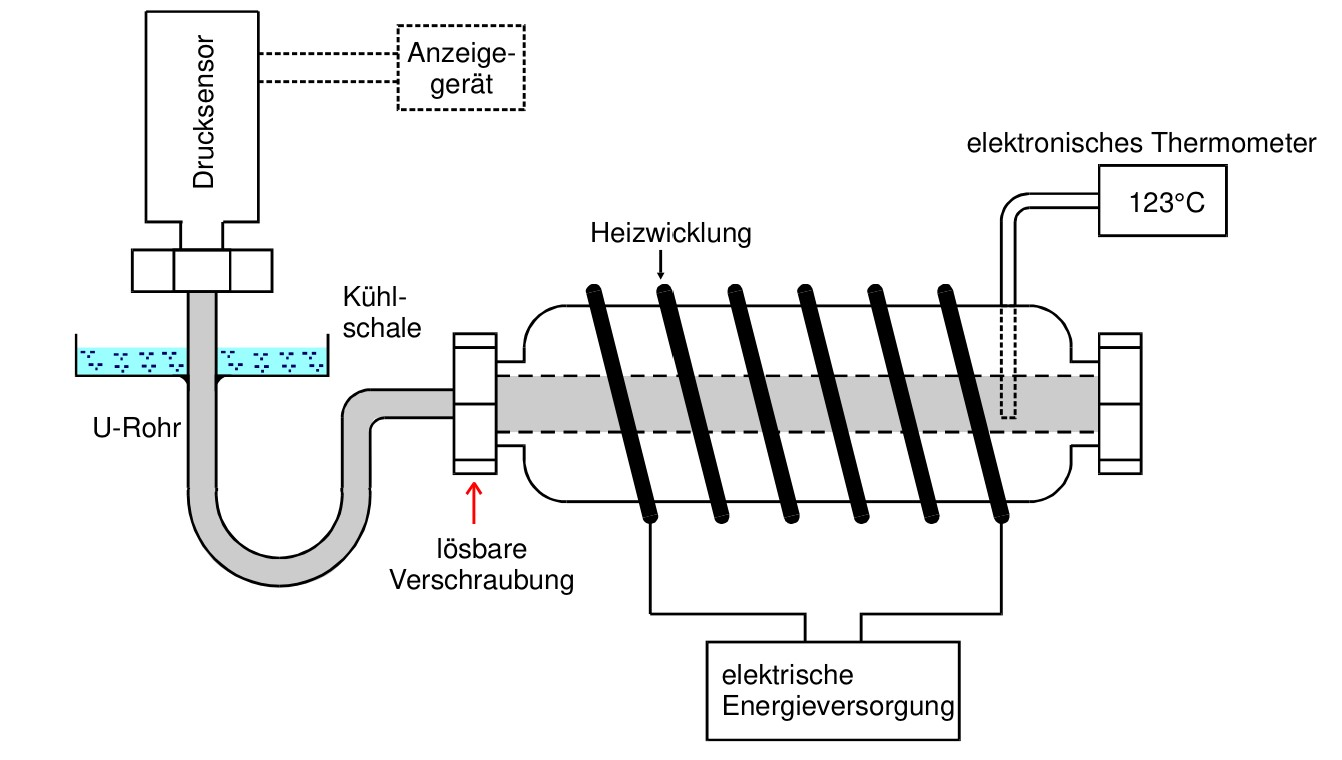
\includegraphics[scale=0.5]{screen3.jpg}
    \caption{Der Versuchsaufbau der zweiten Versuchsreihe als Skizze.\cite{V203_Anleitung}}
\end{figure}
Im zweiten Teil des Versuchs wird eine vergleichbare Messung für den Druckbereich von 1 bis 15\,bar durchgeführt.
Hierfür muss jedoch eine andere Messapparatur verwendet werden, da die zuerst verwendete Glasapparatur dem Druck nicht Stand halten würde.
Diese Apparatur besteht aus einem hohlen Stahlbolzen, welcher sich über einer Heizapparatur befindet.
In dem Hohlraum befindet sich das Wasser.
Die Temperatur des Wassers wird über ein Thermometer angegeben, welches ins Innere des Stahlbolzen ragt.
Anders als in der Anleitung beschrieben wurde hier ein analoges Thermometer genutzt.
Der Druck im Stahlbolzen wird über einen Drucksensor, welcher mit dem Hohlraum verbunden ist, gemessen.
\noindent
Nachdem die Heizung eingeschaltet ist und der Druck durch die Erwärmung des Wassers auf $\SI{1}{\bar}$ angestigen ist, 
beginnt die Messung.
Die Temperatur wird mit steigendem Druck gemessen in Abständen von einem bar, bis ein Druck von $\SI{15}{\bar}$ erreicht ist.